\chapter{Introducción}

\thispagestyle{plain}
\renewcommand{\tablename}{Tabla}

\section{Objeto}
Este Trabajo de Fin de Grado pretende poner de manifiesto los conocimientos adquiridos en el Grado de Ingeniería Electrónica Industrial. Dicho trabajo permite profundizar en alguna/s de las materias desarrolladas en el Grado. 

\section{Antecedentes}

La Robótica de Rescate es un campo emocionante y vital que fusiona la tecnología robótica con el propósito humano de salvar vidas en situaciones de emergencia. Con un enfoque en el diseño, desarrollo y despliegue de robots inteligentes y ágiles, esta disciplina busca proporcionar soluciones innovadoras para enfrentar desafíos en entornos peligrosos o inaccesibles para los equipos de rescate convencionales. Desde terremotos hasta incendios forestales, la Robótica de Rescate ofrece herramientas y sistemas avanzados para mejorar la eficiencia y seguridad en operaciones de salvamento, protegiendo tanto a los rescatistas como a las víctimas.

\subsection{Robótica de Rescate en la UMA}

Entrando en proyectos llevados a cabo en la Universidad de Málaga, encontramos el Laboratorio de Robótica y Mecatrónica, integrado en el Departamento de Ingeniería de Sistemas y Automática (ISA). Entre sus actividades de investigación encontramos la Robótica para catástrofes, búsqueda y rescate y la Robótica de campo.

\begin{figure}[H]
    \centering
    \begin{subfigure}[c]{0.45\textwidth}
        \centering
        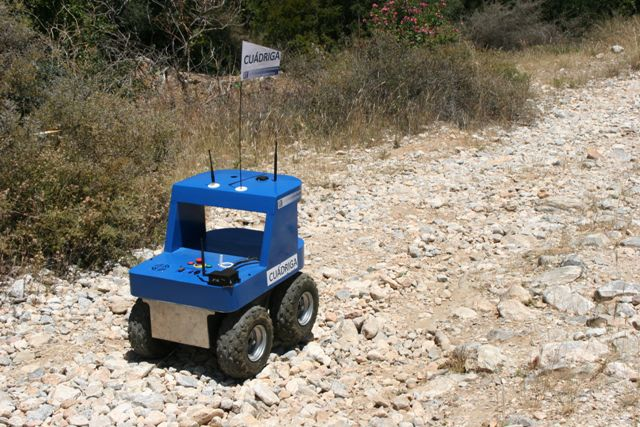
\includegraphics[width = \textwidth]{imagenes/Intro - Cuadriga.jpg}
        \caption{Cuádriga}
        \label{fig:Cuadriga}
    \end{subfigure}
    \begin{subfigure}[c]{0.45\textwidth}
        \centering
        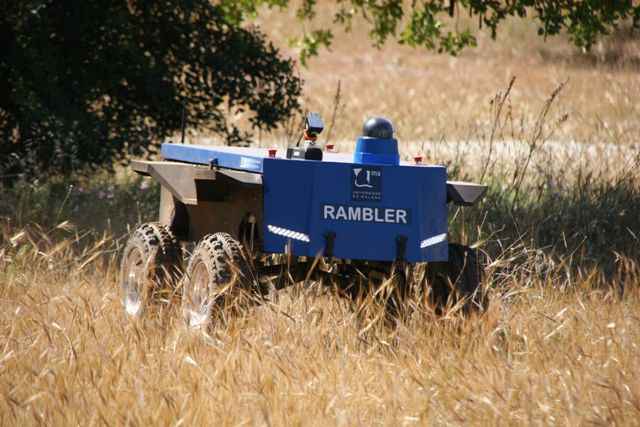
\includegraphics[width = \textwidth]{imagenes/Intro - Rambler.jpg}
        \caption{Rambler}
        \label{fig:Rambler}
    \end{subfigure}
    \caption{Robots del Laboratorio de Robótica y Mecatrónica \cite{RoboticaISA}.}
\end{figure}

%\subsubsection{J8}

%\subsubsection{Cuádriga}

Cuadriga es un robot que cuenta con dirección deslizante, un sistema de control avanzado que se utiliza para mejorar la maniobrabilidad y la estabilidad del vehículo en diversos terrenos. Utiliza motores de corriente continua con escobillas con engranajes de reducción lo cual le permite ejercer un gran par a baja velocidad, con la contraprestación de no poder alcanzar velocidades elevadas.

%\subsubsection{Rambler}

Rambler(DPI2011-22443) (Figura \ref{fig:Rambler}), es un robot explorador del tamaño y la potencia de un vehículo eléctrico, que alcanza una velocidad de 80 kilómetros por hora. Con un peso aproximado de 200 kg, consta de un sistema de amortiguación activa y un brazo manipulador que permite realizar el triaje a las víctimas. Este, se presentó de manera oficial en las VIII Jornadas de Seguridad, Emergencias y Catástrofes acogida en la Escuela de Industriales en el año 2014. 

El sistema de tracción está compuesto por ruedas dotadas de motores de accionamiento directo de corriente continua sin escobillas, más eficientes que los motores del robot. Estos motores permiten una gran velocidad pero presentan el inconveniente de carecer de par necesario para el movimiento a velocidades muy bajas.

Tanto el robot Rambler como el robot Cuádriga, carecen de electrónica de potencia y electrónica de control, que en ambos casos presentan la necesidad de un volumen de espacio considerable dentro del vehículo, a parte del coste adicional que conlleva.

\subsubsection{Donatello v2021}

El robot utilizado en este proyecto, Donatello, es un robot de rescate con el que se participa en la competición RoboCupRescue Robot League. Esta es una liga internacional de equipos con un objetivo: desarrollar y demostrar capacidades robóticas avanzadas para equipos de rescate utilizando competiciones anuales para evaluar y campamentos de enseñanza para difundir las mejores soluciónes robóticas.

En el año 2021 se realizó el primer diseño del robot de rescate Donatello. Este fue realizado por Eva María Góngora Rodríguez \cite{TFG-EV} y Ezequiel Farina \cite{TFG-EZ}. Este diseño presentaba algunas deficiencias, ya que el excesivo cableado y las vibraciones del vehículo provocan la desconexión de cables y por tanto fallos. 

\begin{figure}[H]
    \centering
    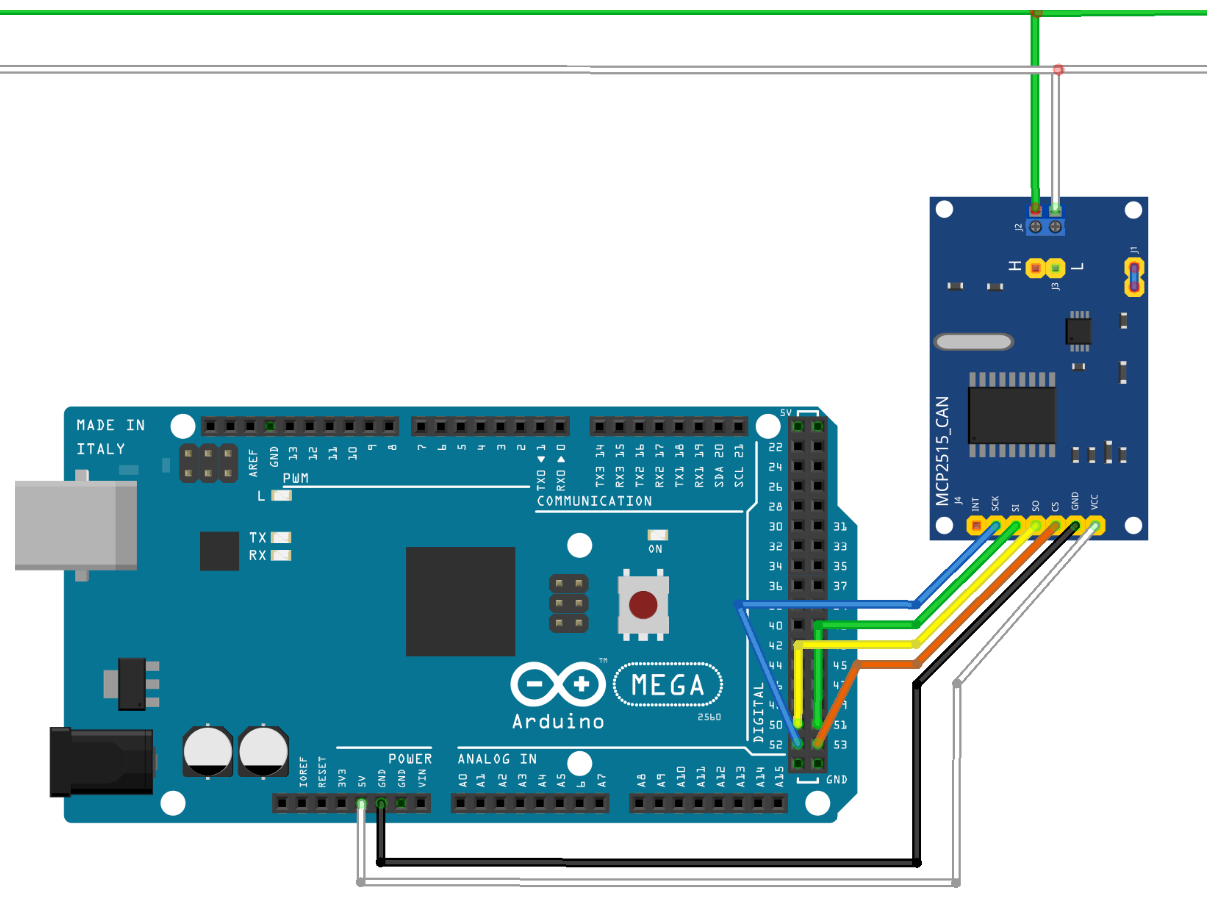
\includegraphics[width=0.5 \linewidth]{imagenes/ConfiguracionAnteriorDonatello.png}
    \caption{Esquema conexión Arduino Mega 2560 y módulo MCP2515. \cite{TFG-EZ}}
    \label{fig:Fritzing-ConexionAnterior}
\end{figure}

La figura \ref{fig:Fritzing-ConexionAnterior} muestra el esquema existente anterior a este proyecto. Se plantea por tanto la sustitución del módulo CAN por una \textit{shield} para el Arduino Mega 2560. Esto hará que el sistema electrónico del vehículo robótico sea más robusto. Reduciendo el número de cables y por tanto el riesgo de una desconexión de estos. También, se estudiará la sustitución de la placa Arduino Mega 2560 por una Arduino MKR con CAN Shield.

\subsection{Motores GIM8108v3 y el MIT Mini Cheetah}

Los motores utilizados en este proyecto (Figura \ref{fig: Motor GIM8108v3}), cuyas características se desarrollan en más profundidad en el capítulo sobre el hardware utilizado, se basan en los del MIT Mini Cheetah (Figura \ref{fig: Motor MIT Mini Cheetah}) cuyo proyecto fue liderado por Benjamin Katz \cite{Katz2016}. 

\begin{figure}[H]
    \centering
    \begin{subfigure}[c]{0.45\textwidth}
        \centering
        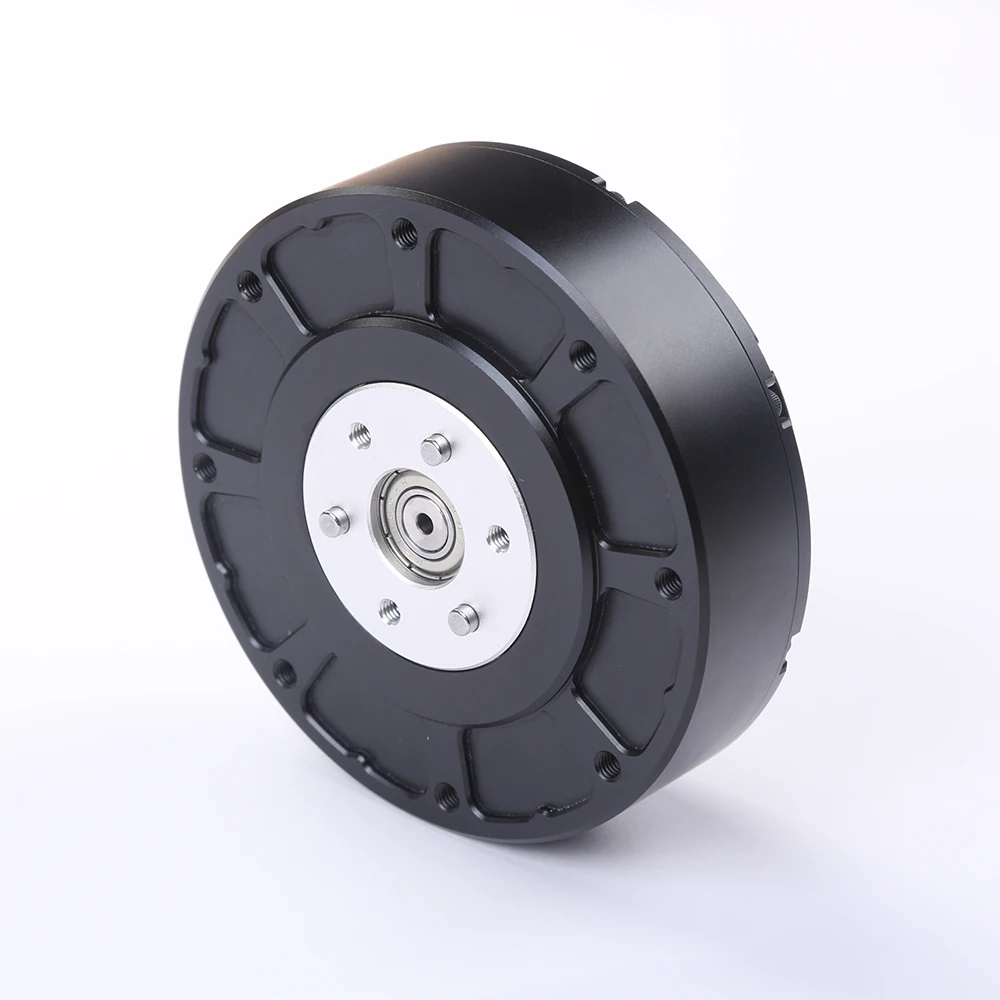
\includegraphics[width=0.75\linewidth]{imagenes/Intro - GIM8108 - Motor.png}
        \caption{Motor GIM8108v3 \cite{GIM8108v3}}
        \label{fig: Motor GIM8108v3}
    \end{subfigure}
    \begin{subfigure}[c]{0.45\textwidth}
        \centering
        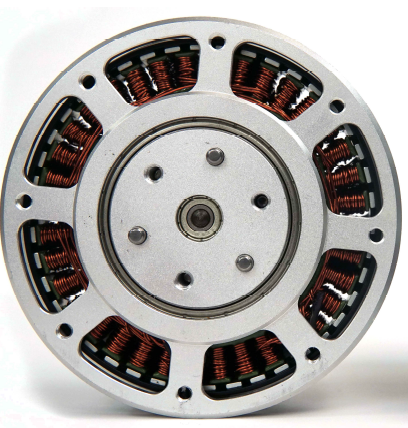
\includegraphics[width=0.75\linewidth]{imagenes/Intro - MIT - Motor.png}
        \caption{Motor MIT \cite{Katz2016}}
        \label{fig: Motor MIT Mini Cheetah}
    \end{subfigure}
    \caption{Motores de MIT y SteadyWin}
\end{figure}

Este robot cuadrúpedo de algo más de 9 kg, destaca por ser robusto, ligero y ágil. Llama la atención su capacidad de levantarse en caso de caer al suelo como si nada hubiera pasado, aparte de ser el primer `robot acróbata' capaz de hacer volteretas.

\begin{figure}[H]
    \centering
    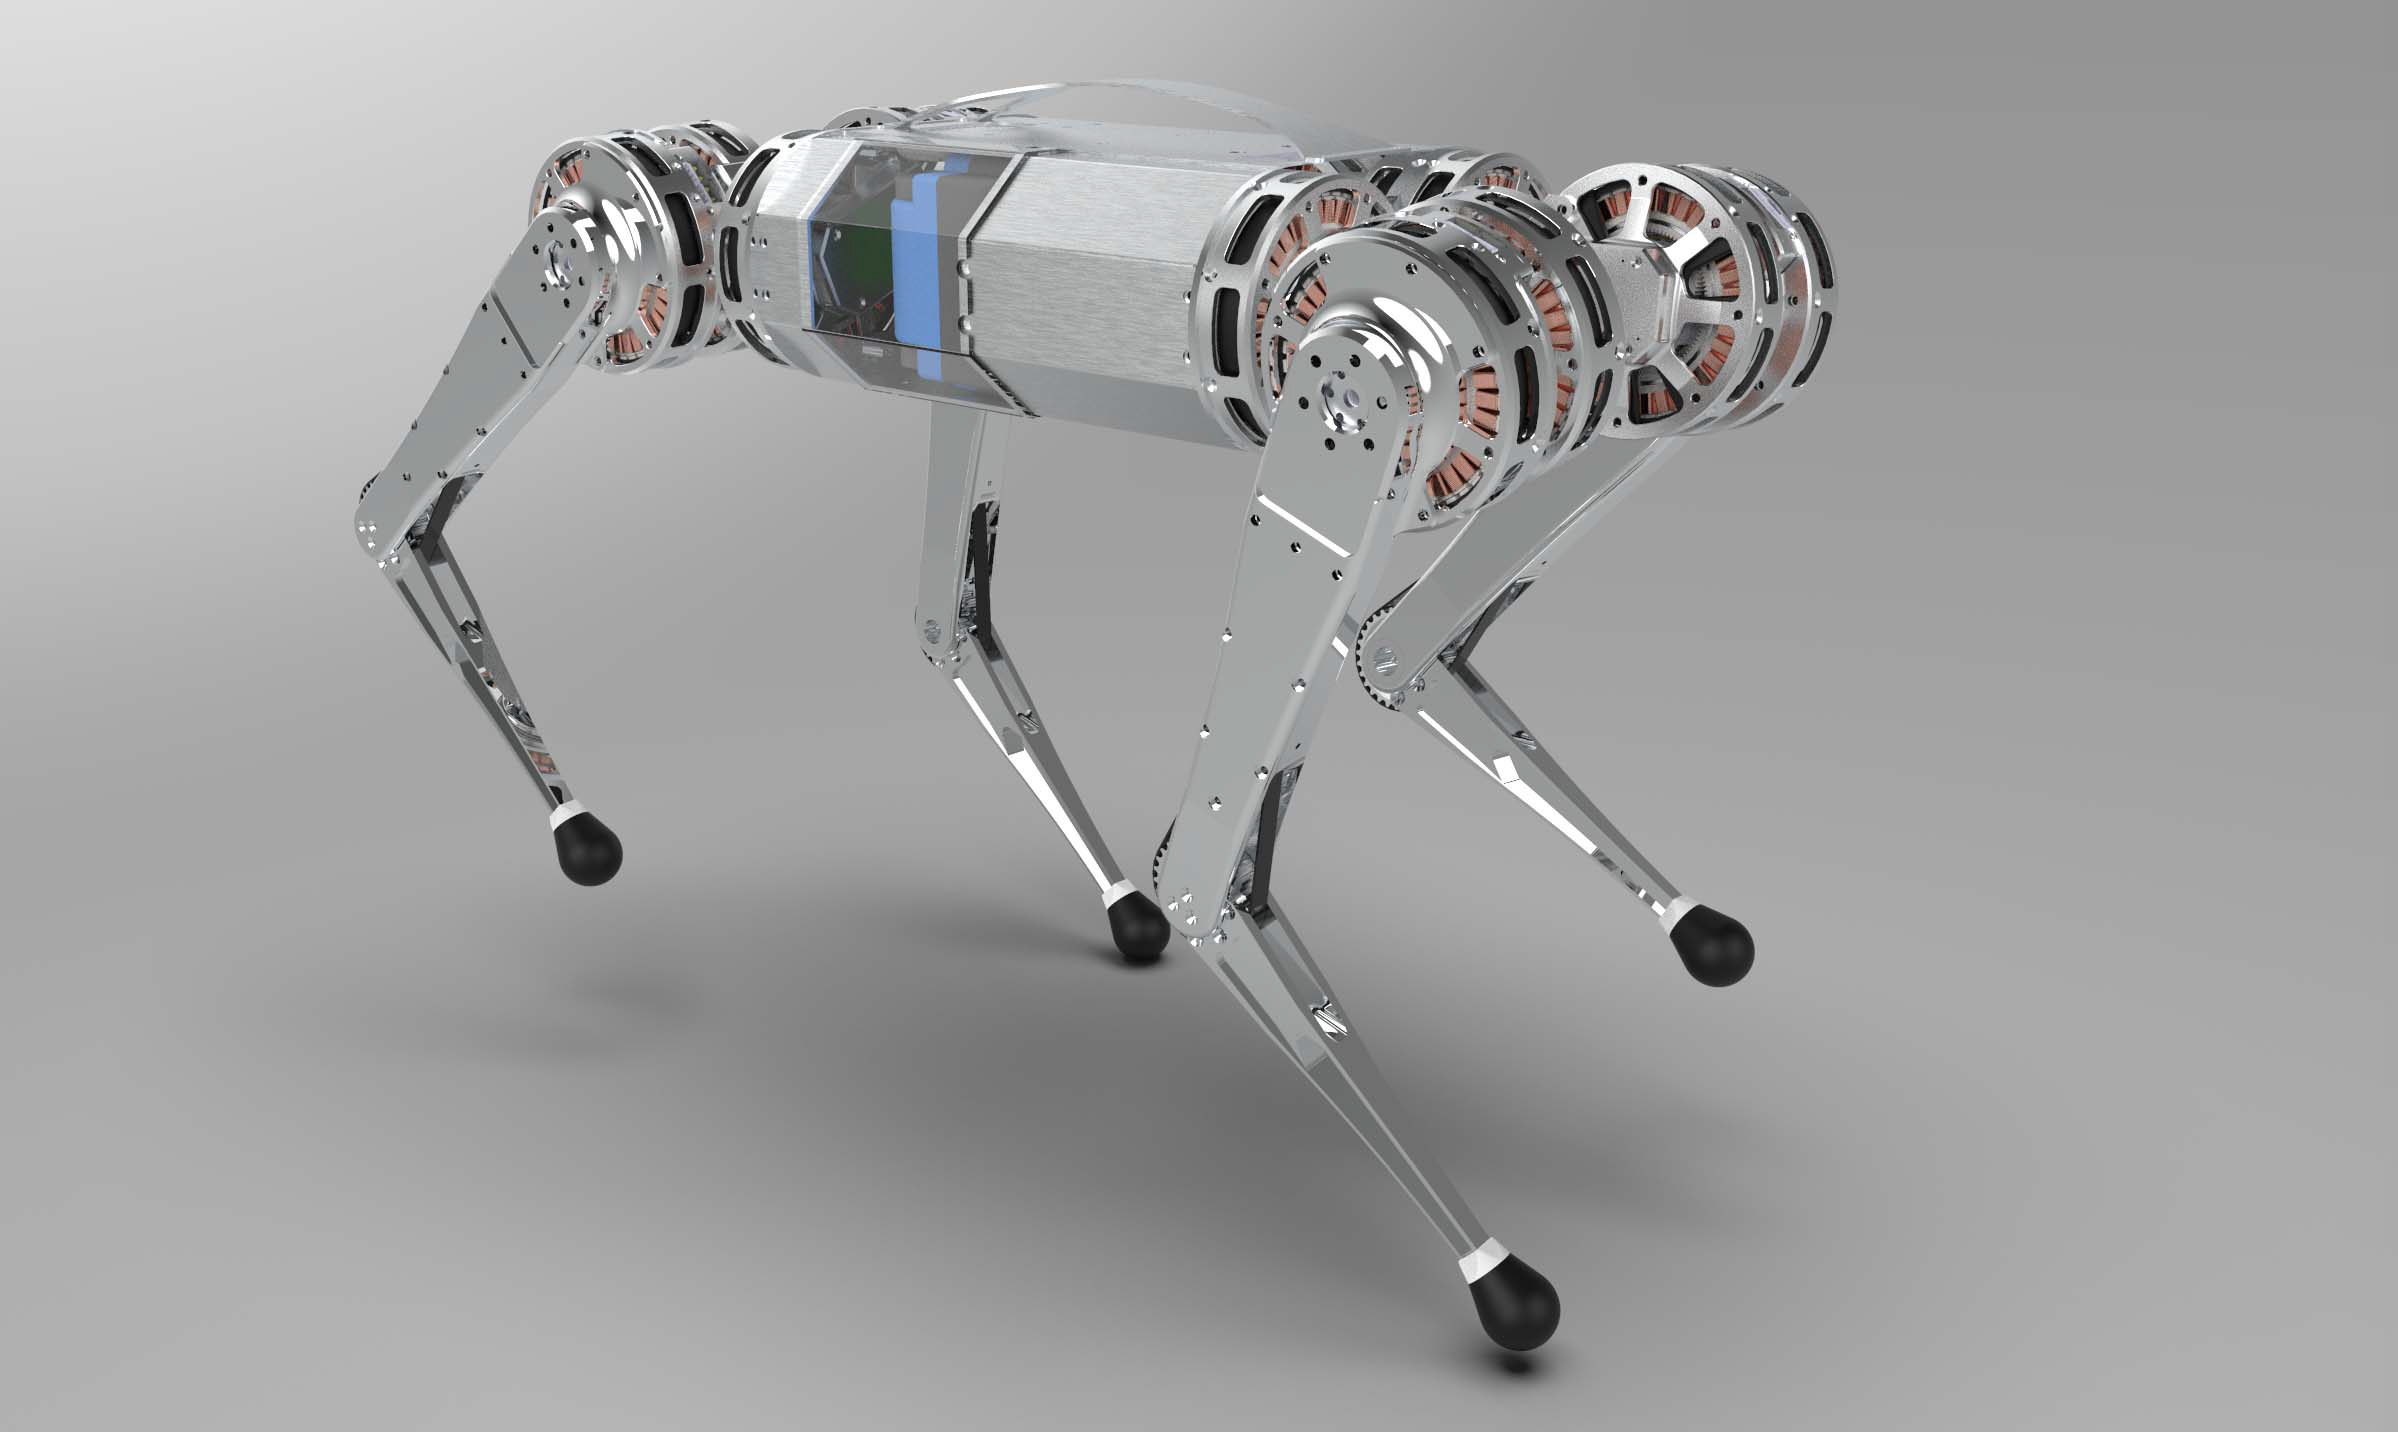
\includegraphics[width=0.75\linewidth]{imagenes/Intro - MIT - Mini Cheetah.png}
    \caption{MIT Mini-Cheetah}
    \label{fig:enter-label}
\end{figure}

Su actuador utiliza el rotor y el estator de un motor sin escobillas comercial diseñado para grandes drones RC. El modelo en particular usado es casi idéntico en forma y rendimiento al T-Motor U8, que se utilizó en el robot Minitaur. Estos motores están integrados en un actuador que también incluye una reductora planetaria de una sola etapa de 6:1 y la electrónica de potencia y de control del motor con sensor de posición incorporado. 

Steadywin ofrece una versión de estos motores, pudiendo elegir entre el controlador de código abierto del MIT (utilizado en este proyecto) y un nuevo controlador SHS.

\section{Objetivo}

El objetivo de este trabajo es implementar, haciendo uso de SIMULINK y una placa Arduino, un controlador para los servomotores del vehículo robótico Donatello. Este robot forma parte del equipo de RoboRescue de la Universidad de Málaga.

\begin{figure}[H]
    \centering
    \begin{subfigure}[c]{0.45\textwidth}
        \centering
        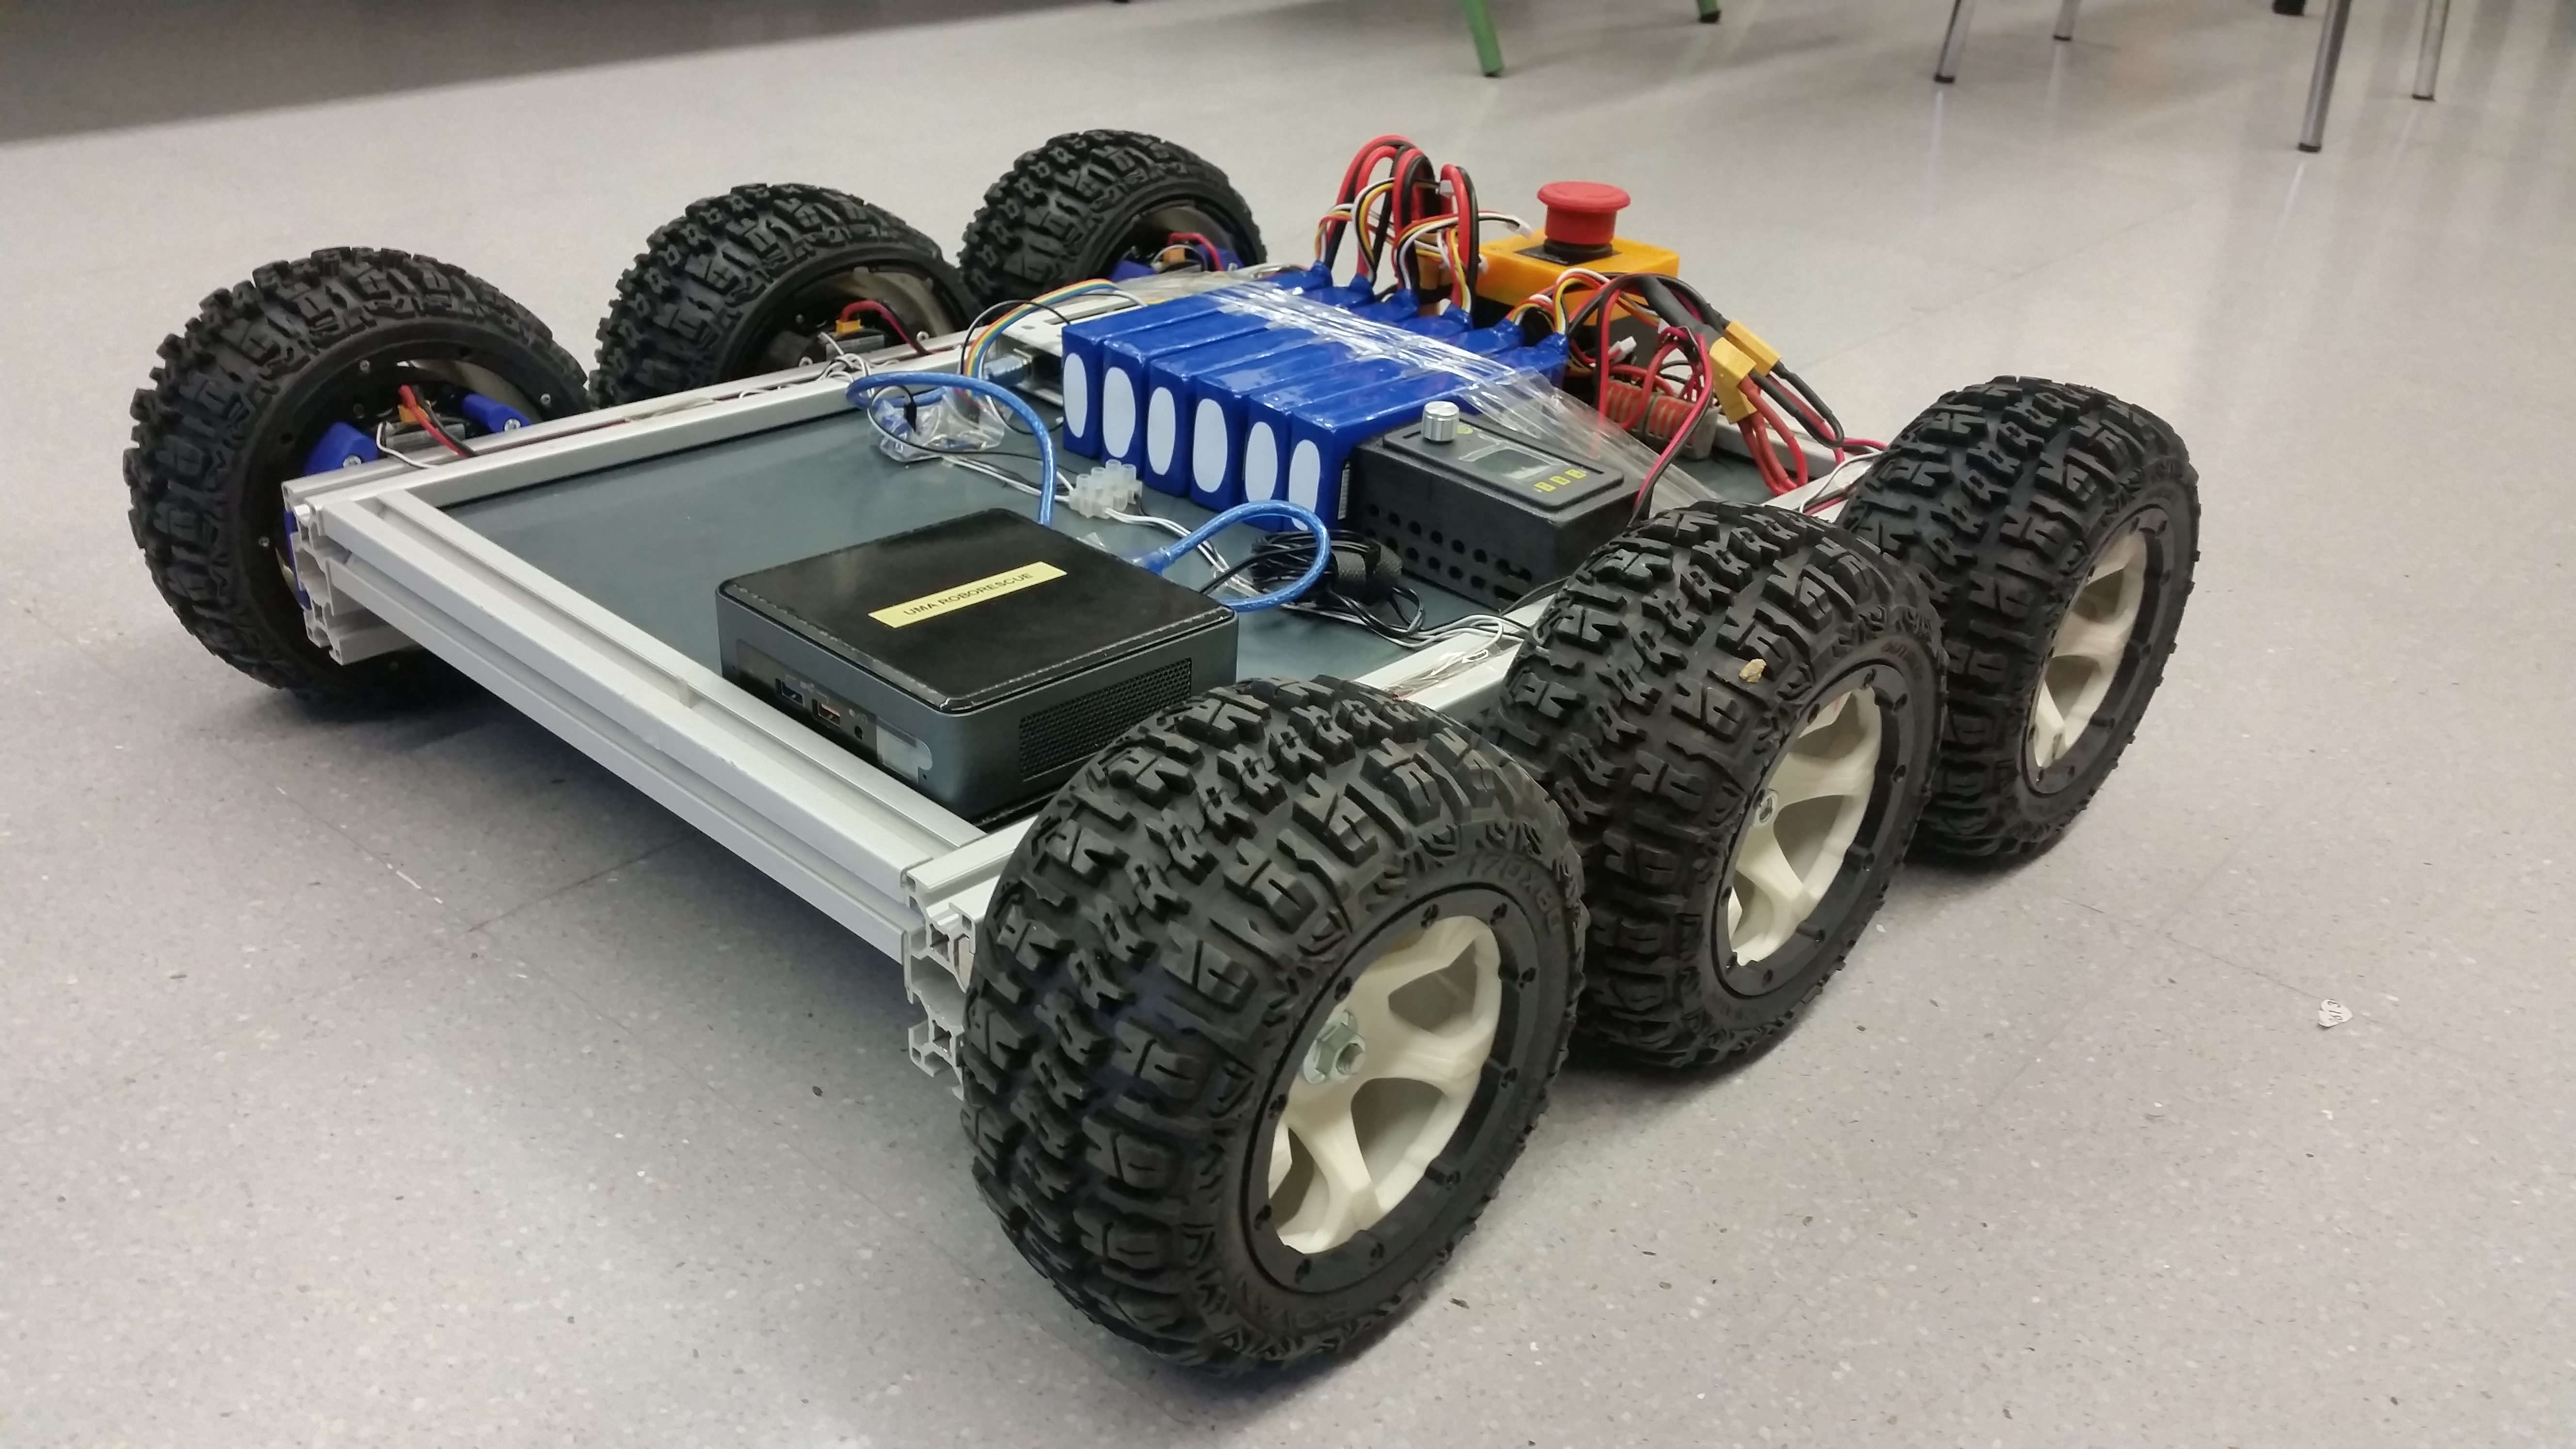
\includegraphics[width = 1\textwidth]{imagenes/Donatello 2021.jpg}
        \caption{Donatello año 2021 \cite{TFG-EV}.}
        \label{fig:Donatello-2021}
    \end{subfigure}
    \hfill
    \begin{subfigure}[c]{0.45\textwidth}
        \centering
        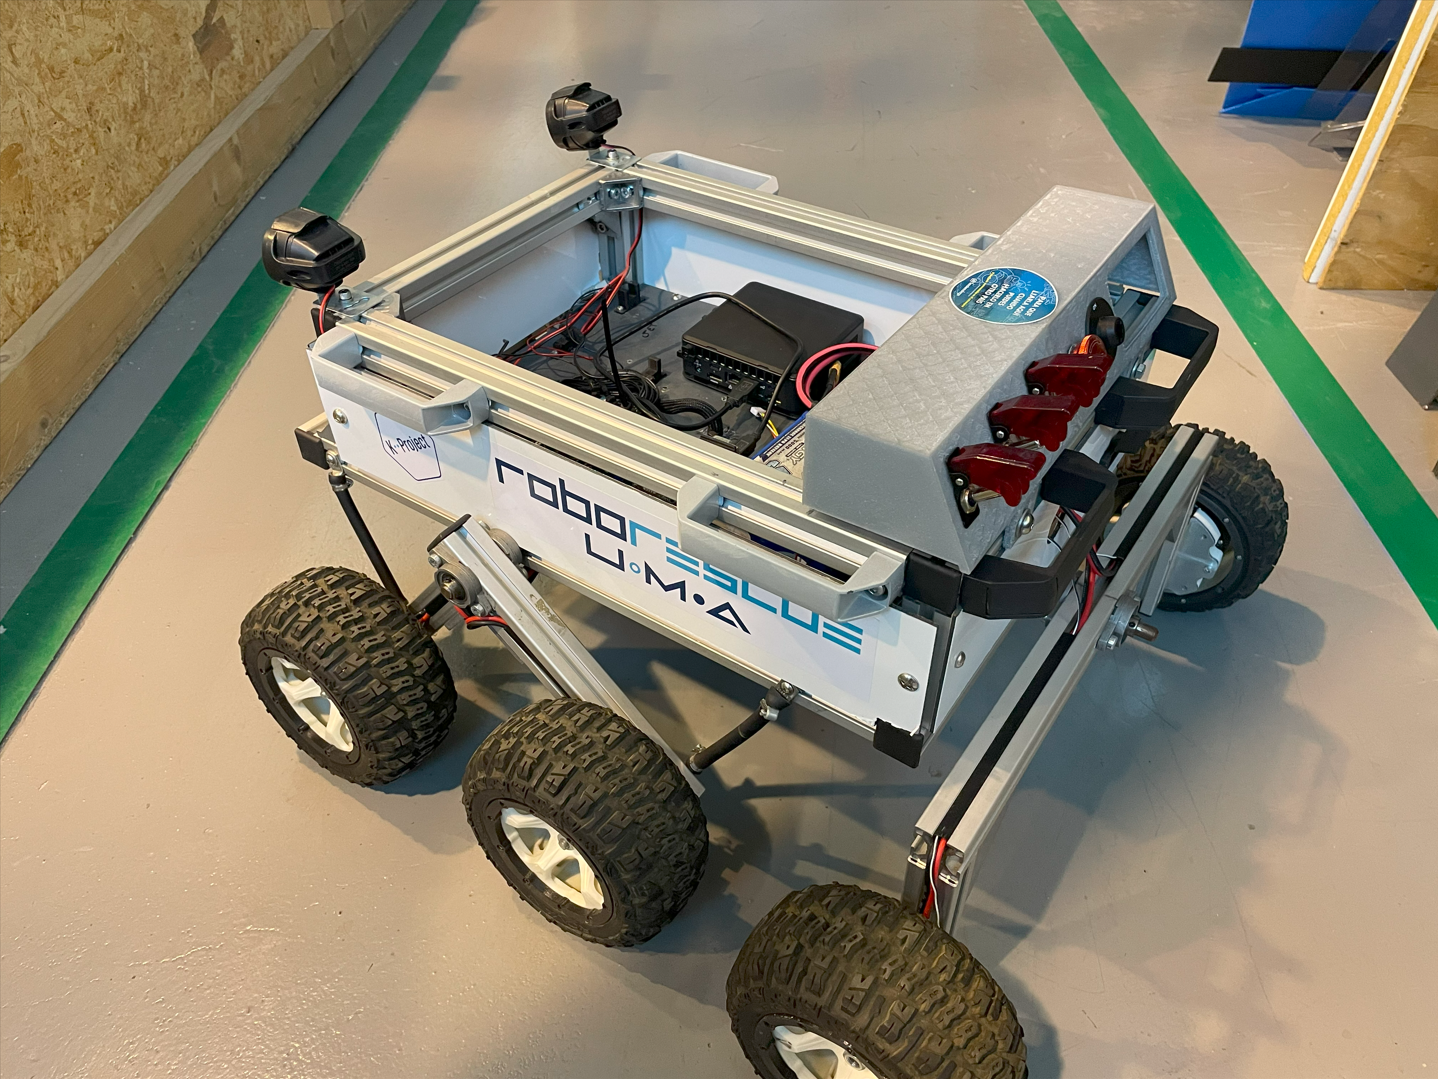
\includegraphics[width = 1\textwidth]{imagenes/Donatello 2024.png}
        \caption{Donatello año 2024.}
        \label{fig:Donatello-2024}
    \end{subfigure}
    \caption{Chasis antiguo y actual del vehículo robótico.}
    \label{fig:DonatelloVersiones}
\end{figure}

\section{Fases del trabajo}

El trabajo tendrá lugar en el taller 0.27.T.II y constará de las siguientes partes:

\begin{enumerate}
    \item Instalación del software y búsqueda bibliográfica: instalación del software que se va a utilizar, como MATLAB, Arduino IDE y SIMULINK, así como de los paquetes específicos necesarios.
    \item Estudio de los motores.
    \item Desarrollo del código de control: se modelará utilizando Simulink.
    \item Realización de pruebas: se comprobará el correcto funcionamiento del modelo diseñado experimentalmente.
    \item Documentación: elaboración de la memoria del trabajo realizado así como de la documentación técnica necesaria.
\end{enumerate}

% \section{¿Por qué es interesante este trabajo?}

\section{Contenido de la memoria}

El documento se divide en ocho capítulos, siendo este capítulo de introducción el primero de la memoria. A continuación se describen brevemente los siete capítulos restantes.

\begin{itemize}
    \item El segundo capítulo se introducirán los componentes del hardware utilizados.
    \item En el tercer capítulo se describe el software utilizado.
    \item El cuarto capítulo explica el control del motor de SteadyWin. Entrando en detalles de la comunicación CAN y su firmware.
    \item El quinto capítulo sirve de introducción a ROS. Comentando en que consiste este middleware y probando su conexión con MATLAB y su correcto funcionamiento simulado en Gazebo.
    \item En el sexto capítulo se describen los subsistemas que integran el modelo de control del vehículo desde el ordenador. Este capítulo se inicia con una introducción a la comunicación en serie ordenador-placa, para posteriormente adentrarse en la explicación de todos los subsistemas que hacen posible este control.
    \item A continuación, en el séptimo capítulo describe los subsistemas que integran el modelo del control del vehículo. Desde su modelo cinemático inverso a modelo cinemático directo, pasando por odometría o control de parámetros.
    \item Por último, en el octavo capítulo, se elaboran las conclusiones obtenidas durante la realización de este trabajo, así como la proposición de mejoras futuras. 
\end{itemize}

Finalmente, se incluye una sección de anexos donde se recogen los distintos códigos usados en este proyecto.

%\blankpage